\documentclass{beamer}
\usepackage{graphicx}
\usepackage[polish]{babel}
\usepackage[utf8]{inputenc}
\usepackage[T1]{fontenc}

\usetheme{Rochester}
\usecolortheme{wolverine}

\title{Co słychać w Perlu 6}
\subtitle{Opowieść o Perlu, Rakudo i wydarzeniach bieżących}
\author{Tadeusz Sośnierz}

\begin{document}
\begin{frame}{Co słychać w Perlu 6}
	\titlepage
\end{frame}

			\section{Wprowadzenie}

\begin{frame}{Dlaczego warto dziś mówić o Perlu 6?}
	\begin{block}{Larry Wall}
		„Perl 5 was my rewrite of Perl. I want Perl 6 to be
		the community's rewrite of Perl
		and of the community.”
	\end{block}
	\pause
	\begin{itemize}
		\item 19 lipca 2000 -- ogłoszenie Perla 6
			-- Równo 10 lat temu!
		\pause
		\item Perl 6 nie jest już tylko specyfikacją
		\pause
		\item Za 10 dni (29 lipca) wydane zostanie Rakudo Star
			-- dystrybucja Perla 6 zdatna do użytku
		\pause
		\item W ten czwartek (22 lipca) zostanie wydane Rakudo \#31,
			na którym będzie oparte Rakudo Star
	\end{itemize}
\end{frame}

\begin{frame}{Camelia}
	\begin{columns}
		\begin{column}{0.5\textwidth}
			
\includegraphics[scale=0.54]{camelia}
		\end{column}
		\begin{column}{0.5\textwidth}
			{\Huge »ö«}
		\end{column}
	\end{columns}
	
\includegraphics[scale=0.38]{newlogo}
\end{frame}

\begin{frame}{Rakudo i Parrot}
	\begin{center}
		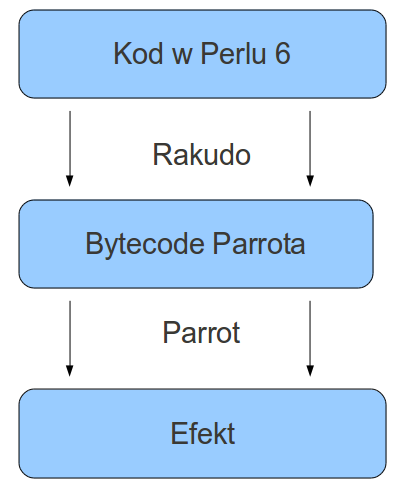
\includegraphics[scale=0.4]{bohomaz}
	\end{center}
\end{frame}
			\section{Co się tam dzieje teraz}
			\subsection{Parrot}

\begin{frame}{Parrot}
	\begin{itemize}
		\item Maszyna wirtualna dla języków dynamicznych
		\item Dostępne implementacje Perla 6, Pythona, Ruby i innych
		\item Wydawana regularnie co miesiąc, jutro (20.07) wersja 2.6.0 
	\end{itemize}
\end{frame}

			\subsection{Rakudo}

\begin{frame}{Rakudo}
	\begin{center}
		
\includegraphics[scale=0.5]{rakudo}
	\end{center}
	\begin{itemize}
		\item (Jap.) „The Way Of The Camel”, tudzież „Paradise”
		\item Kompilator Perla 6 w Perlu 6
		\item Również wydawany co miesiąc, dwa dni po wydaniu Parrota
		\item Aktualnie spełnia około 83\% testów ze specyfikacji
	\end{itemize}
\end{frame}

\begin{frame}{Rakudo -- postęp}
	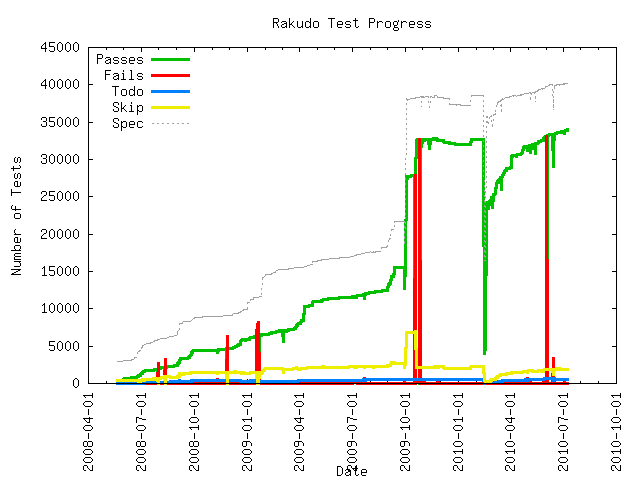
\includegraphics[scale=0.3785]{progress}
\end{frame}

			\subsubsection{Rakudo Star}

\begin{frame}{Rakudo Star}
	\begin{itemize}
		\item „useful and usable”
		\item Nie będzie to kompletna implementacja, ale zdatna do użytku
		\item Ma przyciągnąć uwagę i zachęcić do portowania modułów i pisania kodu
		\item Planowane wydanie -- 29 lipca br.
	\end{itemize}
\end{frame}

\begin{frame}{Rakudo Star}
	A wraz z nim:
	\begin{itemize}
		\item Parrot
		\item Blizkost (o nim za chwilę)
		\item Moduły
		\begin{itemize}
			\item Zavolaj (native call interface)
			\item MiniDBI (subset DBI)
			\item ...
		\end{itemize}
	\item „The Perl 6 Book”
		(\htmladdnormallink{http://github.com/perl6/book}
		{http://github.com/perl6/book})
	\end{itemize}
\end{frame}

			\subsection{Powiązane}
\begin{frame}[fragile]{Blizkost}
	Daje możliwość używania Perla 5 jako jednego z języków
	w Parrocie, co pozwala nam używać modułów z Perla 5
	w kodzie w Perlu 6
	\begin{block}{blikost/examples/cgi.pl}
\begin{verbatim}
use v6;
use CGI:from<perl5>;
my $q = CGI.new;

print $q.header, $q.start_html('Hello World'),
      $q.h1('Hello World'), $q.end_html;
\end{verbatim}
	\end{block}
\end{frame}

\begin{frame}[fragile]{Zavolaj}
	„Wołanie” funkcji z C bezpośrednio w Perlu 6
	\begin{block}{zavolaj/examples/sqlite3.p6 (fragmenty)}
\begin{verbatim}
use NativeCall;
sub sqlite3_open( Str $filename, OpaquePointer $ppDB )
    returns Int
    is native('libsqlite3')
    { ... }

my OpaquePointer $db;
my $status = sqlite3_open("test.db", $db);
\end{verbatim}
	\end{block}
\end{frame}

\begin{frame}{Moduły -- proto, pls}
	\begin{itemize}
		\item proto -- instalator modułów Perla 6
		\item nowy projekt: pls (ma zastąpić proto)
		\item \htmladdnormallink{http:/modules.perl6.org}
			{http:/modules.perl6.org} -- baza modułów
		\begin{itemize}
			\item Math::Model
			\item MiniDBI
			\item LWP::Simple
			\item SVG
			\item ufo
			\item URI
			\item XML, XML::Writer
			\item Web
			\item HTTP::Server::Simple, HTTP::Server::Simple::PSGI (niedostępne w proto)
		\end{itemize}
	\end{itemize}
\end{frame}

\begin{frame}{Inne implementacje}
	\begin{itemize}
		\item PUGS (nierozwijany)
		\item YAPSI -- Yet Another Perl Six Implementation
			(\htmladdnormallink{http://github.com/masak/yapsi}
			{http://github.com/masak/yapsi})
		\item Niecza -- kompilator Perla 6 pod .NET/Mono (\htmladdnormallink{http://github.com/sorear/niecza}{http://github.com/sorear/niecza})
		\item Bennu -- kompilator Perla 6 pod LLVM (\htmladdnormallink{http://github.com/ekiru/Bennu}{http://github.com/ekiru/Bennu})
	\end{itemize}
\end{frame}
			\section{Co się zmieniło}

\begin{frame}{Zmiany, zmiany, zmiany}
	\begin{center}
	{\huge Co się zmieniło w samym języku?}
	\end{center}
\end{frame}

\begin{frame}{Czego nie lubimy w Perlu 5}
	\begin{itemize}
		\item Surowego OOP
		\item Dostępu do parametrów w funkcjach
		\item Łapania wyjątków
		\item Momentami nienajpiękniejszej składni (referencje)
	\end{itemize}
\end{frame}

\begin{frame}{Co się zmieniło}
	\begin{itemize}
		\item OOP -- wszystko jest obiektem, nowa składnia
			tworzenia klas (podobna do tej z MooseX::Declare)
		\item Regexpy, na inne, niekompatybilne z tymi z Perla 5,
			acz o dużo większych możliwościach
		\item Składnia -- miejscami uproszczona,
			ale i dodane mnóstwo nowych elementów
	\end{itemize}
\end{frame}

\begin{frame}[fragile]{Co się zmieniło}
	\begin{center}
		{\Huge Ale to wciąż Perl}
	\end{center}
\end{frame}

\begin{frame}[fragile]{Jakich modułów nie będziemy już potrzebować}
	% czyli jakich ficzerów nie musimy sobie dorabiać, bo mamy je w standardzie
	\begin{itemize}
		\item Moose
		\item Try::Tiny
		\item Data::Dumper -- każda zmienna ma metodę .perl
		\item Devel::REPL -- REPLa mamy w standardzie
		\item Getopt::* -- możemy ustalić listę parametrów
			dla funkcji MAIN (o tym wkrótce) %TODO
	\end{itemize}
\end{frame}
			\subsection{Typowanie}
\begin{frame}[fragile]{Typowanie}
	Jest możliwość nadania zmiennej typu

	\begin{semiverbatim}
\alert{> my Int \$a = 5; \$a = "foo"}
Type check failed for assignment
	\end{semiverbatim}

	\begin{semiverbatim}
\alert{> my Str \$a = "foo"; \$a = 5}
Type check failed for assignment
# ale...
\alert{> my Str \$a = "foo"; \$a = 5.Str; \$a.perl.say}
"5"
	\end{semiverbatim}
	\begin{semiverbatim}
\alert{> say ~[5.WHAT, 'string'.WHAT, (3/7).WHAT, /foo .*/.WHAT]}
Int() Str() Rat() Regex()
	\end{semiverbatim}
\end{frame}

			\subsection{Wszystko jest obiektem}

\begin{frame}[fragile]{Wszystko jest obiektem}
	\begin{semiverbatim}
\alert{> 'a string'.\^\relax{}methods.sort[40..45]}
bytes can capitalize ceiling chars chomp
\alert{> "the big brown fox".split(' ').grep(/\^\relax{}b/).join(' and ')}
big and brown
	\end{semiverbatim}
\end{frame}
			\subsection{Prefixy zmiennych}
\begin{frame}{Prefixy zmiennych}
		W Perlu 6 prefix zmiennej (sigil) nie zmienia się przy wydobywaniu pojedynczego elementu
	\vskip15pt
	\begin{tabular}{l|l}
	Perl 5 & Perl 6 \\
	\hline
	\hline
	my @arr = (1, 2, 3) & my @arr = (1, 2, 3) \\
	my \$elem = \alert{\$arr}[1] & my \$elem = \alert{@arr}[1] \\
	\hline
	my \%hash = (foo => 'bar') & my \%hash = (foo => 'bar') \\
	my \$elem = \alert{\$hash}\{'foo'\} & my \$elem = \alert{\%hash}\{'foo'\} \\
	\end{tabular}
\end{frame}
			\subsection{Wszystko jest referencją}
\begin{frame}[fragile]{Wszystko jest referencją}
	Nie ma rozróżnienia na zmienne i referencje do nich,
	a więc nie ma już problemów z dereferowaniem tychże.
	\begin{verbatim}
my $a = { foo => [1, 2, 3] }
	\end{verbatim}
	\begin{columns}[t]
		\begin{column}{0.5\textwidth}
			\begin{block}{Perl 5}
				\begin{verbatim}
push @{ $href->{foo} }, 4
				\end{verbatim}
			\end{block}
		\end{column}
		\begin{column}{0.5\textwidth}
			\begin{block}{Perl 6}
				\begin{verbatim}
$a<foo>.push: 4
# albo $a<foo>.push(4)
				\end{verbatim}
			\end{block}
		\end{column}
	\end{columns}
{\scriptsize(Podczas prezentacji podany przykład był nieco inny,
zmieniłem go aby podkreślić efekt)}
\end{frame}
			\subsection{Funkcje i parametry}
\begin{frame}[fragile]{Funkcje i parametry}
	\begin{verbatim}
sub foo (Str $what, Int $times = 1) {
    say $what x $times
}

foo "hello", 5; # hellohellohellohellohello
foo "hello";    # hello
foo;            # Not enough positional parameters passed;
                # got 0 but expected between 1 and 2
	\end{verbatim}
\end{frame}
			\subsection{Funkcja MAIN}
\begin{frame}[fragile]{Funkcja MAIN}
\small
\begin{verbatim}
sub MAIN($v?, :$arg!, :$arg2 = 'wartość domyślna') {
    if ($v) { # verbose
        say "Zaczynamy"
    }
    say "arg: $arg, arg2: $arg2"
}
\end{verbatim}
\begin{semiverbatim}
\$ \alert{perl6 main.pl}
Usage:
./main.pl [--arg2=value-of-arg2] --arg=value-of-arg [v]

\$ \alert{perl6 main.pl -v --arg=5}
Zaczynamy
arg: 5, arg2: wartość domyślna

\$ \alert{perl6 main.pl --arg=5 --arg2=foo}
arg: 5, arg2: foo
\end{semiverbatim}
\end{frame}
			\subsection{Junctions}
\begin{frame}[fragile]{Junctions}
	\begin{semiverbatim}
\alert{> say 'ok' if 5 == any(3, 5, 7) # albo 5 == 3 | 5 | 7}
ok
\alert{> say 'ok' if 5 == none(4, 6, 8)}
ok
\alert{> my Junction \$x = 3 | 5; say 'ok' if \$x == 5}
ok
\alert{> my @scores = 32, 41, 73, 99, 52;
> say 'ok' if all(@scores) > 30;}
ok
	\end{semiverbatim}
\end{frame}
			\subsection{Laziness}
\begin{frame}[fragile]{Laziness}
	\begin{semiverbatim}
\alert{> my \$even = (2, 4 ... *); \$even[\^\relax{}10].perl.say}
(2, 4, 6, 8, 10, 12, 14, 16, 18, 20)
\alert{> my \$sq = gather for 0..Inf \{ take \$\_ * \$\_ \}; \$sq[5].say}
25
	\end{semiverbatim}
\end{frame}
			\subsection{Try-CATCH}
\begin{frame}[fragile]{Try-CATCH}
\begin{verbatim}
try {
    die "Oh noes!";
    CATCH {
        say "Something went wrong: $_";
    }
}
\end{verbatim}
\end{frame}
			\subsection{OOP -- Perl 6 a Moose}
\begin{frame}[fragile]{OOP}
\begin{columns}[t]
	\begin{column}{0.5\textwidth}
	\begin{block}{Perl 5 z Moose}
{\tiny
\begin{verbatim}
package Point;
use Moose;

has ['x','y'] => (is => 'rw', isa => 'Int');

sub clear {
    my $self = shift;
    $self->x(0);
    $self->y(0);
}

package Point3D;
use Moose;
extends 'Point';

has 'z' => (is => 'rw', isa => 'Int');

after 'clear' => sub {
    my $self = shift;
    $self->z(0);
};
\end{verbatim}
}
	\end{block}
	\end{column}
	\begin{column}{0.5\textwidth}
	\begin{block}{Perl 6}
{\tiny
\begin{verbatim}
class Point {

  has Int $.x is rw;
  has Int $.y is rw;

  method clear {
    $.x = $.y = 0;
  }

}

class Point3D is Point {

  has Int $.z is rw;

  method clear {
    nextsame;
    $.z = 0;
  }

}
\end{verbatim}
}
	\end{block}
	\end{column}
\end{columns}
\end{frame}
			\subsection{Gramatyki}
\begin{frame}[fragile]{Gramatyki}
\tiny
\begin{verbatim}
grammar URI {
    token TOP {
        <schema> '://' 
        [<hostname> | <ip> ]
        [ ':' <port>]?
        '/' <path>?
    }
    token byte {
        (\d**{1..3}) <?{ $0 < 256 }>
    }
    token ip {
        <byte> [\. <byte> ] ** 3
    }
    token schema {
        \w+
    }
    token hostname {
        (\w+) ( \. \w+ )*
    }
    token port {
        \d+
    }
    token path {
        <[ a..z A..Z 0..9 _\-.!~*'():@&=+$,/ ]>+
    }
}
my $match = URI.parse('http://perl6.org/documentation/');
say $match<hostname>;  # perl6.org
say $match<path>;      # documentation
\end{verbatim}
\end{frame}

			\section{Co teraz?}
\begin{frame}{Co możemy zrobić teraz}
	Co możemy zrobić poza bezczynnym czekaniem na Rakudo Star?
	\begin{itemize}
		\item Pisać kod, szukać bugów
		\item Robić pozytywny szum o Perlu 6 :)
	\end{itemize}
\end{frame}
			\section{Linki}

\begin{frame}{Linki}
	\begin{itemize}
		\item \htmladdnormallink{http://perl6.org/}
			{http://perl6.org/}
		\item \htmladdnormallink{http://parrot.org}
			{http://parrot.org}
		\item \htmladdnormallink{http://rakudo.org}
			{http://rakudo.org}
		\item
		\htmladdnormallink{http://perlgeek.de/en/article/5-to-6}
		{http://perlgeek.de/en/article/5-to-6}
		-- wprowadzenie do Perla 6 dla programistów Perla 5
		
		\item \htmladdnormallink{http://perl6advent.wordpress.com/}
			{http://perl6advent.wordpress.com/}
			-- Perl 6 Advent Calendar, cykl ciekawych artykułów o
			nowościach w Perlu 6
		\item Kanał \#perl6 na irc.freenode.net
	\end{itemize}
\end{frame}

\end{document}
